\fancyhead[L]{\textbf{\textsf{28}}\quad\textbf{\textsf{\color{stewartcyan}CHƯƠNG 1}}\quad\textsf{Hàm số và Mô hình}}
\fancyhead[R]{}

\noindent
\begin{minipage}[t]{0.26\textwidth}
    \vspace{2.3cm}
    \raggedright
    \textbf{\textsf{HÌNH 13}}\\
    {\small Đồ thị của các hàm căn}
\end{minipage}%
\hfill
\begin{minipage}[t]{0.71\textwidth}
    \noindent
    parabol $x = y^2$. [Xem Hình 13(a).] Đối với các giá trị chẵn khác của $n$, đồ thị của $y = \sqrt[n]{x}$ tương tự như đồ thị của $y = \sqrt{x}$. Với $n = 3$, ta có hàm căn bậc ba $f(x) = \sqrt[3]{x}$ có tập xác định là $\mathbb{R}$ (hãy nhớ rằng mọi số thực đều có một căn bậc ba) và đồ thị của nó được thể hiện trong Hình 13(b). Đồ thị của $y = \sqrt[n]{x}$ với $n$ lẻ ($n > 3$) tương tự như đồ thị của $y = \sqrt[3]{x}$.

    \vspace{0.25cm}
    \begin{center}
        \begin{minipage}[b]{0.48\textwidth}
            \centering
            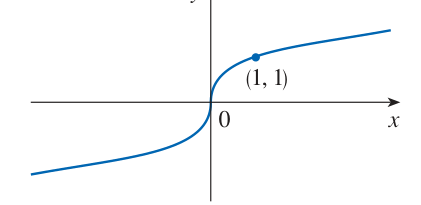
\includegraphics[width=0.9\linewidth]{images/p0063_fig1.png}
        \end{minipage}\hfill
        \begin{minipage}[b]{0.48\textwidth}
            \centering
            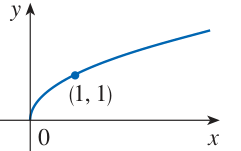
\includegraphics[width=0.9\linewidth]{images/p0063_fig2.png}
        \end{minipage}
    \end{center}

    \vspace{0.16cm}
    \noindent
    {\bfseries\textsf{\color{stewartcyan}(iii) $\boldsymbol{a = -1}$}}

    \vspace{0.12cm}
    \noindent
    Đồ thị của \textbf{hàm nghịch đảo} $f(x) = x^{-1} = 1/x$ được biểu diễn trong Hình 14. Đồ thị của nó có phương trình $y = 1/x$, hay $xy = 1$, và là một hyperbol nhận các trục tọa độ làm các đường tiệm cận. Hàm số này xuất hiện trong vật lý và hóa học liên quan đến Định luật Boyle, phát biểu rằng khi nhiệt độ không đổi, thể tích $V$ của một khối khí tỉ lệ nghịch với áp suất $P$:
    \[
    V = \frac{C}{P}
    \]
    trong đó $C$ là một hằng số. Do đó đồ thị của $V$ theo biến $P$ (xem Hình 15) có dạng hình học tương tự như nhánh bên phải của Hình 14.

    \vspace{0.25cm}
    \begin{center}
        \begin{minipage}[t]{0.48\textwidth}
            \centering
            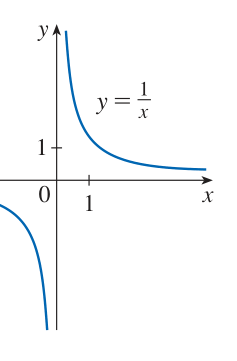
\includegraphics[width=0.85\linewidth]{images/p0063_fig3.png}\\[2mm]
            \raggedright
            \textbf{\textsf{HÌNH 14}}\\
            {\small Hàm nghịch đảo}
        \end{minipage}\hfill
        \begin{minipage}[t]{0.48\textwidth}
            \centering
            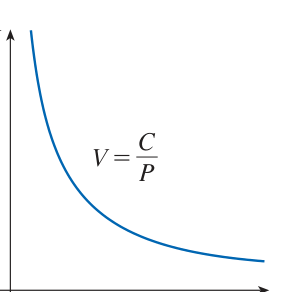
\includegraphics[width=0.85\linewidth]{images/p0063_fig4.png}\\[2mm]
            \raggedright
            \textbf{\textsf{HÌNH 15}}\\
            {\small Thể tích dưới dạng một hàm theo áp suất ở nhiệt độ không đổi}
        \end{minipage}
    \end{center}

    \vspace{0.16cm}
    \noindent
    {\bfseries\textsf{\color{stewartcyan}(iv) $\boldsymbol{a = -2}$}}

    \vspace{0.12cm}
    \noindent
    Trong các số mũ âm còn lại của hàm lũy thừa $f(x) = x^a$, trường hợp quan trọng nhất là $a = -2$. Rất nhiều định luật tự nhiên phát biểu rằng một đại lượng tỉ lệ nghịch với bình phương của một đại lượng khác. Nói cách khác, đại lượng thứ nhất được mô hình hóa bởi một hàm có dạng $f(x) = C/x^2$ và ta gọi đây là một \textbf{định luật nghịch đảo bình phương}. Chẳng hạn, độ rọi sáng $I$ của một vật thể bởi một nguồn sáng tỉ lệ nghịch với bình phương khoảng cách $x$ từ vật đến nguồn sáng:
    \[
    I = \frac{C}{x^2}
    \]
\end{minipage}